\section{Border Gateway Protocol (BGP) Security}

Why should we care about BGP security when we have secure connections (TLS, VPN, DNSSEC, etc.)? The one that controls BGP controls routing.

\begin{itemize}
	\item Obtain fake TLS certs: use BGP route hijacking in combination with automatic certificate issuance (ACME) to obtain fake TLS certs. BGP allows to reroute HTTP challenge traffic from CA to illegitimate IP.
	\item deanonymize TOR users: reroute TOR exit node traffic and use it for correlation attacks.
	\item hijack DNS requests: hijack routes to DNS servers (e.g. MyEtherwallet hack)
	\item Not all traffic is enrypted/authenticated: DNS, HTTP
	\item Even encrypted traffic leaks timing information (fingerprinting)
\end{itemize}

The problem with BGP is that endusers can't protect themselves. Solving these issues is only possible with ISP cooperation.

\subsection{IP Addresses, Autonomous Systems \& the Border Gateway Protocol}

\textbf{IP addresses:} are globally assigned by ICANN (global authority). ICANN assigns certain IP regions to certain parts of the world. Regional Internet Registries (RIRs) are then responsible to further assign IPs. As of 25th November 2019 15:35 UTC+1, we have officially run out of IPv4 addresses.\\
IP addresses are assigned in prefixes (e.g. /16 prefix has $2^{32-16} - 2= 65534)$ IPs).\\

\textbf{Internet:} The Internet is a network of networks (autonomous systems). Autonomous systems can be ISPs (e.g. DT, Swisscom), global backbone network (e.g. Verizon), universities and large companies (e.g. ETH, Google).\\

\textbf{BGP:} BGP "glues" the internet together: routing protocol between ASes, disseminates information about location and paths for IP prefixes. BGP is a path-vector protocol and follows typical business relationships.\\
BGP speaker sends and receives messages from peers over TCP connections on port 179. Messages sent include: \texttt{OPEN, UPDATE, KEEPALIVE, NOTIFICATION}. Route information is disseminated through \texttt{UPDATE} message using attributes: \texttt{Withdraw, path attributes, network layer reachability information}.\\
\\
\paragraph{BGP Policies: }ASes have different business relationships with each other: provider, peer, customer. Each AS implements peering policies. These decide routes are accepted and advertised based on policies. Policies are configured in the BGP daemons of the AS. Policies can be used to implement filters to prevent route leaks (= falsely announced prefixes), or for business reasons.

\begin{itemize}
	\item Input policy: which paths to keep/ discard
	\item Export policy: which paths do I advertise to neighbors
\end{itemize}

\paragraph{How to create your own ISP:}
\begin{enumerate}
    \item Register an autonomous system number to be able to connect via BGP to other networks
    \item Request Internet number resources from your regional network coordination center (get assigned IPv4 and IPv6 prefixes which can be announced over BGP)
    \item Find other networks to connect to and exchange traffic with
    \item Deploy hardware to the peering location an announce IP prefixes
\end{enumerate}

\subsection{BGP Hijacking}
\textbf{BGP vs. OSPF:} BGP is used as an inter Autonomous System protocol, while OSPF is used to establish routes inside an AS. Also, OSPF is a link-state protocol: routers exchange what they know about the network until all routers have a complete map of the network; then the routers compute the routing tables independently. In BGP, we have a path-vector mechanism: every AS announces the prefixes it owns and all the paths that go through it to neighboring ASes.

\begin{minipage}{\linewidth}
    \centering      
    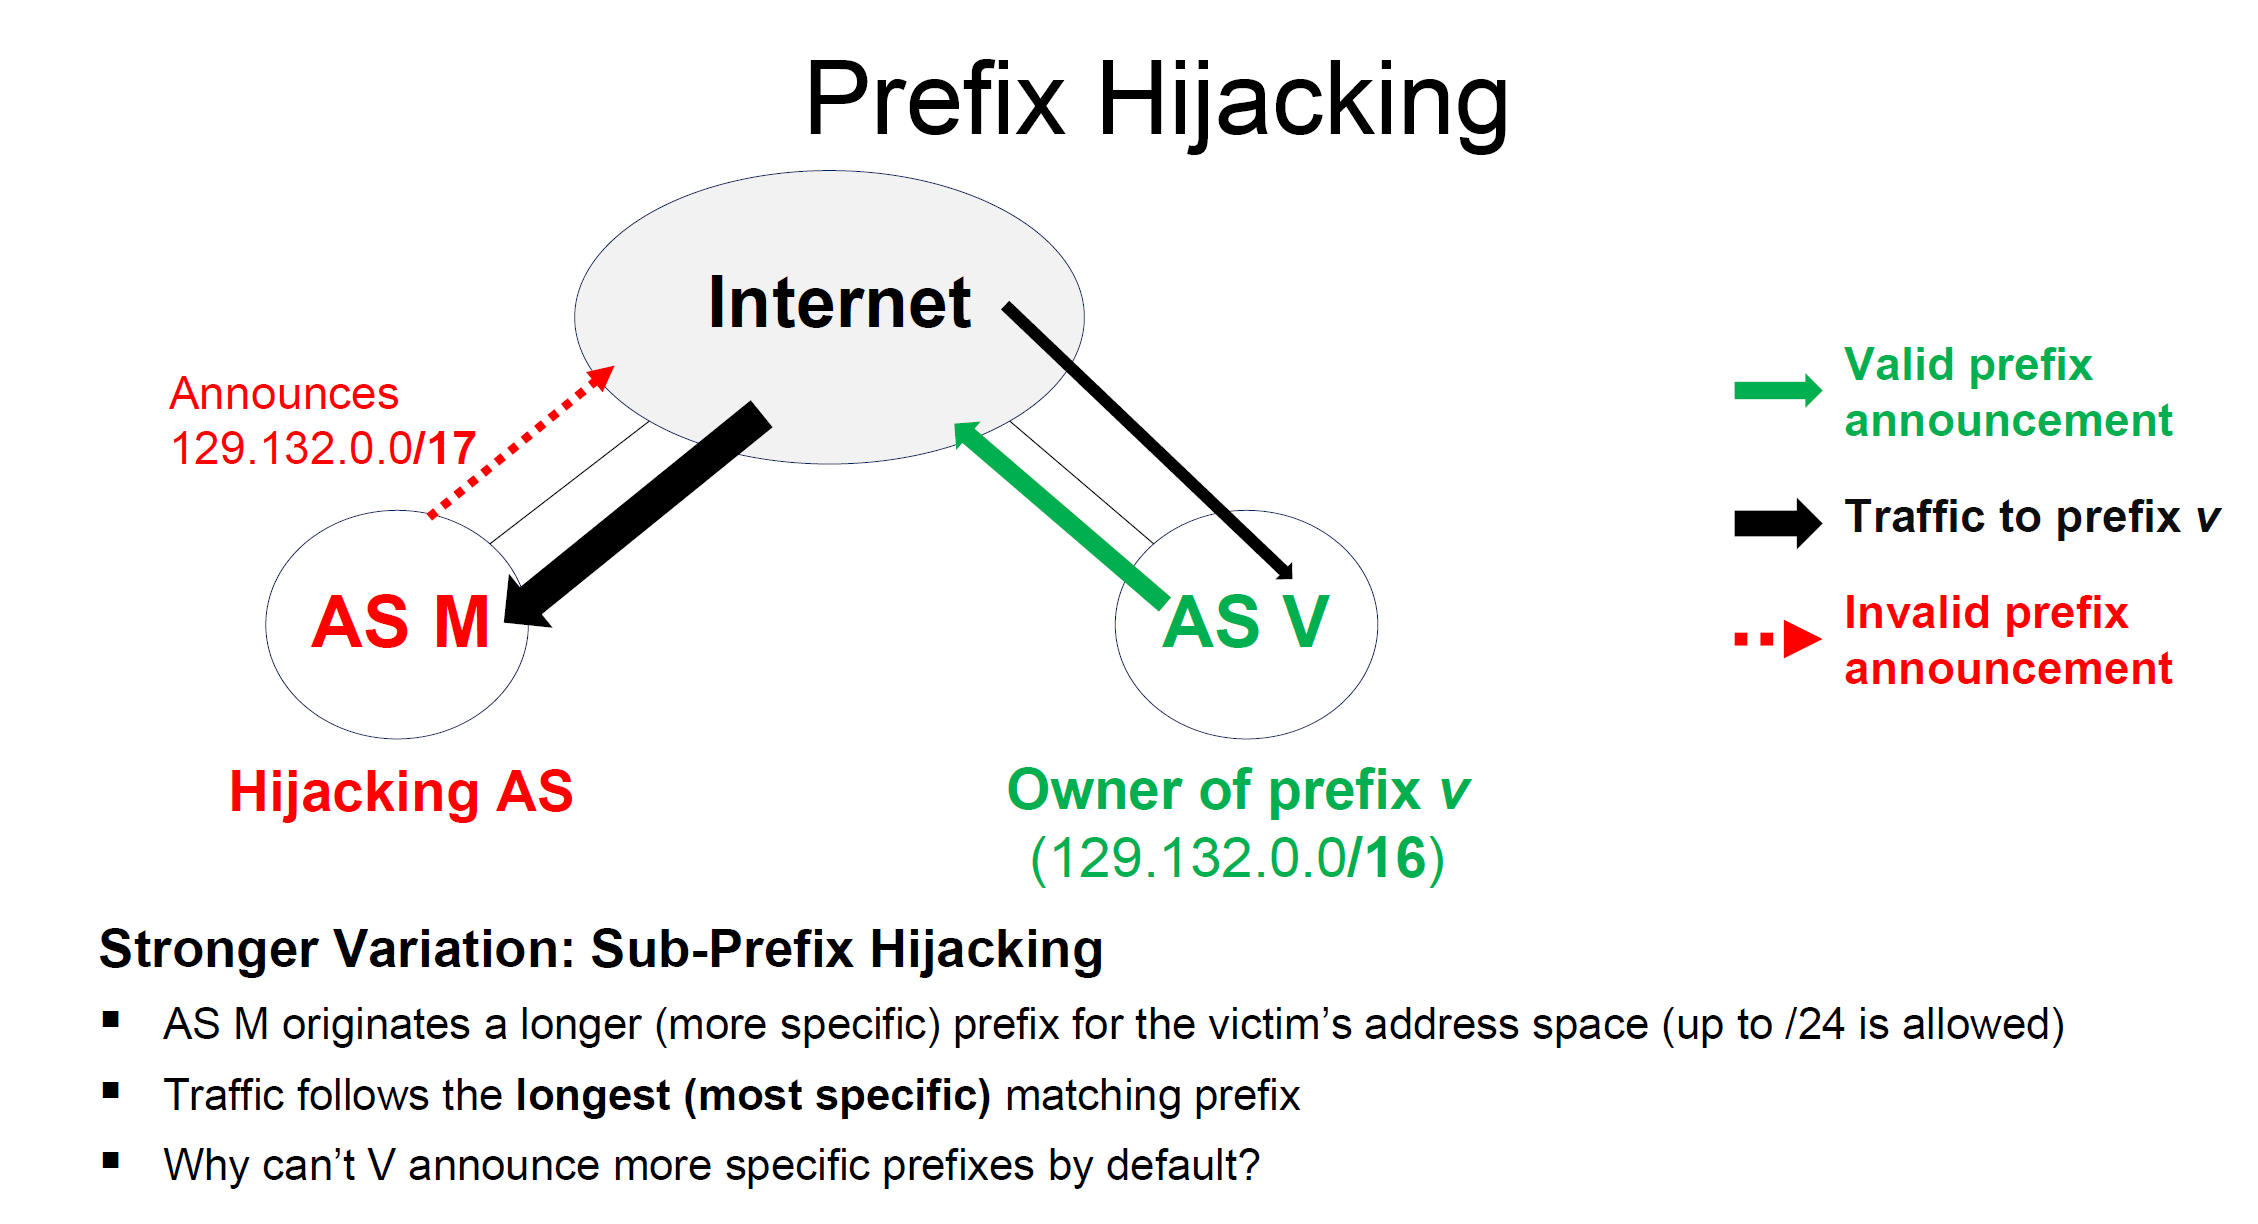
\includegraphics[width=\linewidth]{Figures/BGP_prefix_highjacking.PNG} 
\end{minipage}

Also a less strong attack could be done, where attacker announces same size prefix and only a fraction of traffic to prefix is hijacked. Number of affected sources depends on business relationships, topology, policies.

\subsubsection{Problem 1: BGP does not validate the origin of advertisements!}

\paragraph{IP prefix origination into BGP:} Prefix advertised by the AS who owns the prefix or by upstream providers on its behalf.

\paragraph{IP prefix hijacking:} A malicious or misconfigured AS originates a prefix it does not own, as there is no proper verification in place.

\paragraph{How to perform BGP interception:}
\begin{itemize}
	\item Selective announcement of hijacked prefix only to some neighbors (problem: neighbors may still learn hijacked routes from their peers)
	\item Use BGP poisoning, only select neighbors that use hijacked route.
	\item Use BGP communities to explicitly state to which ASes a particular advertisement should be advertised. Can tell an AS not to forward announcement to specific other ASes using the NoExportSelect action.
\end{itemize}

\paragraph{BGP hijacking in 3 steps:}
\begin{enumerate}
    \item Set up an AS and border router or compromise someone else's router.
    \item Configure router to originate the target (sub-)prefix
    \item Get other ASes to accept the wrong route (Many ASes do not discard wrong routes)
\end{enumerate}
BGP hijacking is not as easy as it sounds (you can't just announce route from your home router). You need access to a BGP router (your own AS or compromised AS).

\subsubsection{Problem 2: BGP does not validate the content of	advertisements}

After a BGP message has been announced, the content of the advertisement is not validated! ASes that receive the advertisement can modify it!

\textbf{ASes can modify the BGP path:}
\begin{itemize}
	\item Remove ASes from the AS path:\\
	Legitimate AS Path: [AS 701, AS 6939, AS 88]. Remove AS 6939: [AS 701, AS 88]\\
	\textbf{Motivation:}
	\begin{itemize}
		\item 	Attract traffic by making path look shorter, attract sources that try to avoid\\
		AS 6939.
	\end{itemize}
	Only AS 701 can tell that the AS path is wrong!
	\item Add ASes to the AS path:\\
	Legitimate AS Path: [AS 701, AS 88]. Add 6939 in-between: [AS 701, AS 6939, AS 88]\\
	\textbf{Motivation:}
	\begin{itemize} 
		\item Trigger loop detection in AS 6939 (AS sees itself on the AS path and drops the advertisement to avoid routing loops) $\rightarrow$ DoS attack on AS 6939, "BGP poisoning".
		\item Make your AS look like it has richer connectivity
	\end{itemize}
	AS 701 can detect the AS path is wrong (but may not care), AS 6939 could detect but may not see the route.
\end{itemize}

\subsection{Attacks on BGP: Obtaining fake certificates}

When using ACME (Automated Certificate Management Environment), a domain is validated through either a HTTP challenge or a DNS challenge to prove that you actually own the domain. By using BGP hijacking, an attacker can:

\begin{minipage}{\linewidth}
    \centering      
    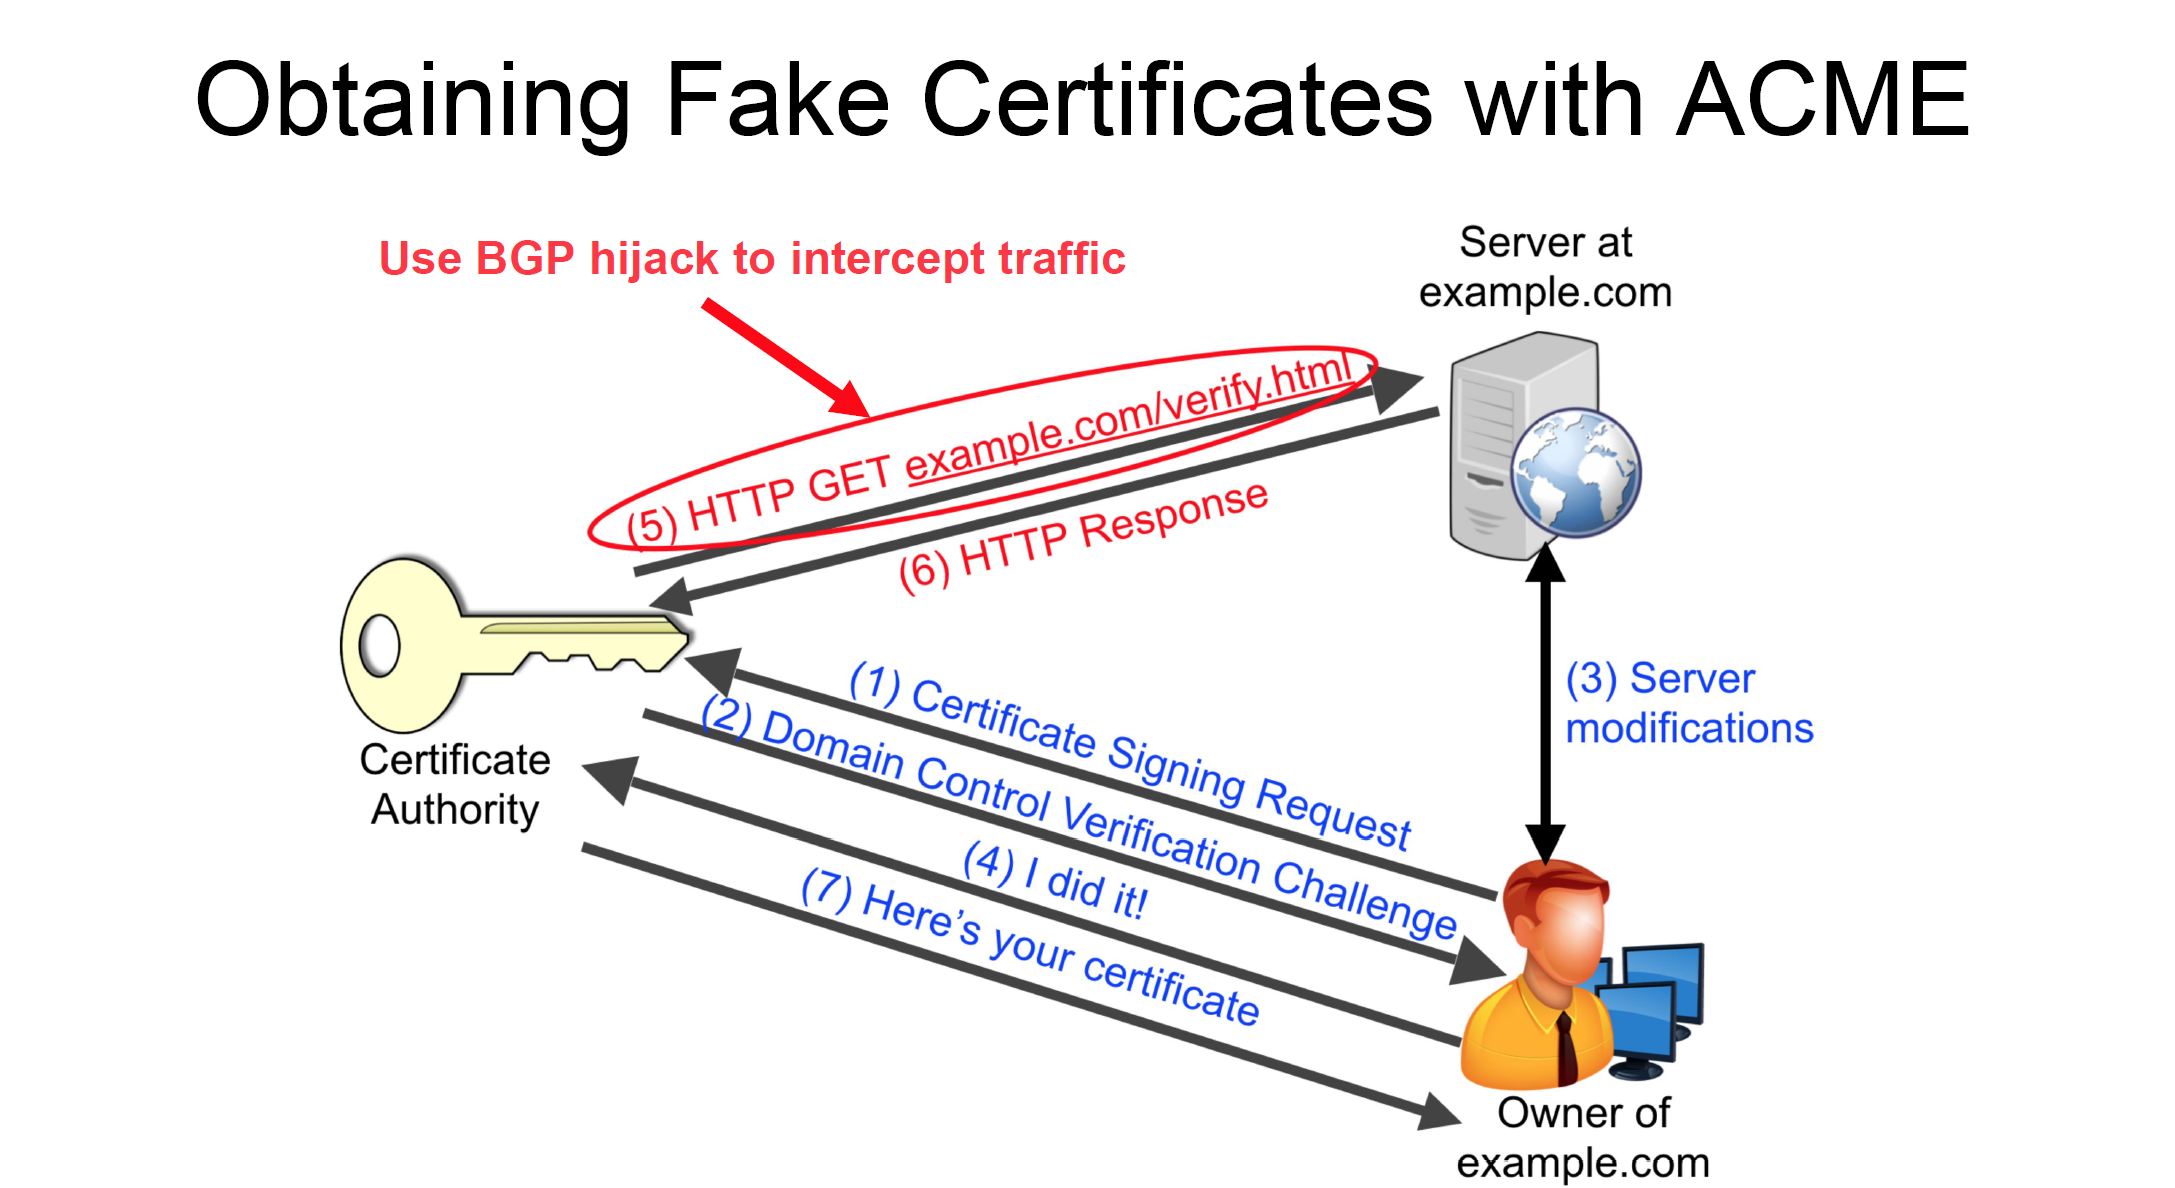
\includegraphics[width=\linewidth]{Figures/BGP_fake_certificates.PNG} 
\end{minipage}

\begin{itemize}
	\item hijack the DNS request of the CA $\rightarrow$ the CA will get a wrong IP owned by the attacker.
	\item hijack the connection to the correct IP and route it to an IP she owns.
\end{itemize}

\subsection{Other attacks on BGP}

\begin{itemize}
	\item Denial-of-service attacks: overload links between BGP routers, send bogus TCP packets (FIN/RST to close session, TCP SYN flood)\\
	A possible solution to bogus TCP RST is to only accept TCP RST with TTL=255, i.e. only TCP RST from direct neighbor router.
	\item Eavesdrop or tamper messages by tapping the link
	\item Most such attacks are easy to defend against and are no longer a large concern
\end{itemize}

\subsection{Countermeasures}
\paragraph{What properties do we want?}
\begin{enumerate}
    \item Only an AS that owns an IP prefix is allowed to announce it (can be proven cryptographically)
    \item Routing messages are authenticated by all ASes on the path (AS cannot add or remove other ASes in BGP announcements)
\end{enumerate}

\subsubsection{Best Current Practices (BCPs)}

\begin{itemize}
	\item Securing the BGP peering session between routers (authentication, prioritize BGP traffic)
	\item Filtering routes by prefix and AS path
	\item Filters to block unexpected control traffic (e.g. ignore TCP RST for BGP if it comes from the inside, implement TTL=255 policy)
	\item Enter prefixes into Internet Routing Registries (IRRs) and filter based on these entries
\end{itemize}

None of these actually have strong security properties (no crypto).

\subsubsection{Solution to Problem 1: Origin Authentication (OA)}
\begin{itemize}
    \item Required: Ability to prove ownership of resources.
    \item Resource Public-Key Infrastructure (RPKI): A secure database to map Internet number resources to a trust anchor. A digital certificate proves that an AS is the current holder of a specific resource. Each regional Internet registry (RIR) is a root of trust.
    \item Enables issuance of Route Origination Authorizations (ROAs): States which AS is authorized to announce certain IP prefixes. Can determine the max length of the prefix that the AS is allowed to advertise (avoid sub-prefix hijacking). Certificate follow same delegation as IP addresses from RIRs
    \item Requires no actual modification to BGP (out-of-band checking)
    \item Trusted local caches collect information from RPKI servers and whitelists are periodically pushed to routers: the verification of signatures is therefore performed offline.
\end{itemize}

If AS M now tries to hijack AS V's prefix $v$, routers will check against ROAs in RPKI for prefix $v$ and see that the announcement is invalid and thus drop it.\\
\textbf{However OA is not enough:} AS M can announce that it has a path to AS V by appending itself on the path \textit{after} the entry for AS V. BGP routers in other ASes check against ROAs in RPKI for prefix $v$, and find a valid ROA for prefix $v$. AS M manages to attract a fraction of traffic for AS V.

\begin{minipage}{\linewidth}
    \centering      
    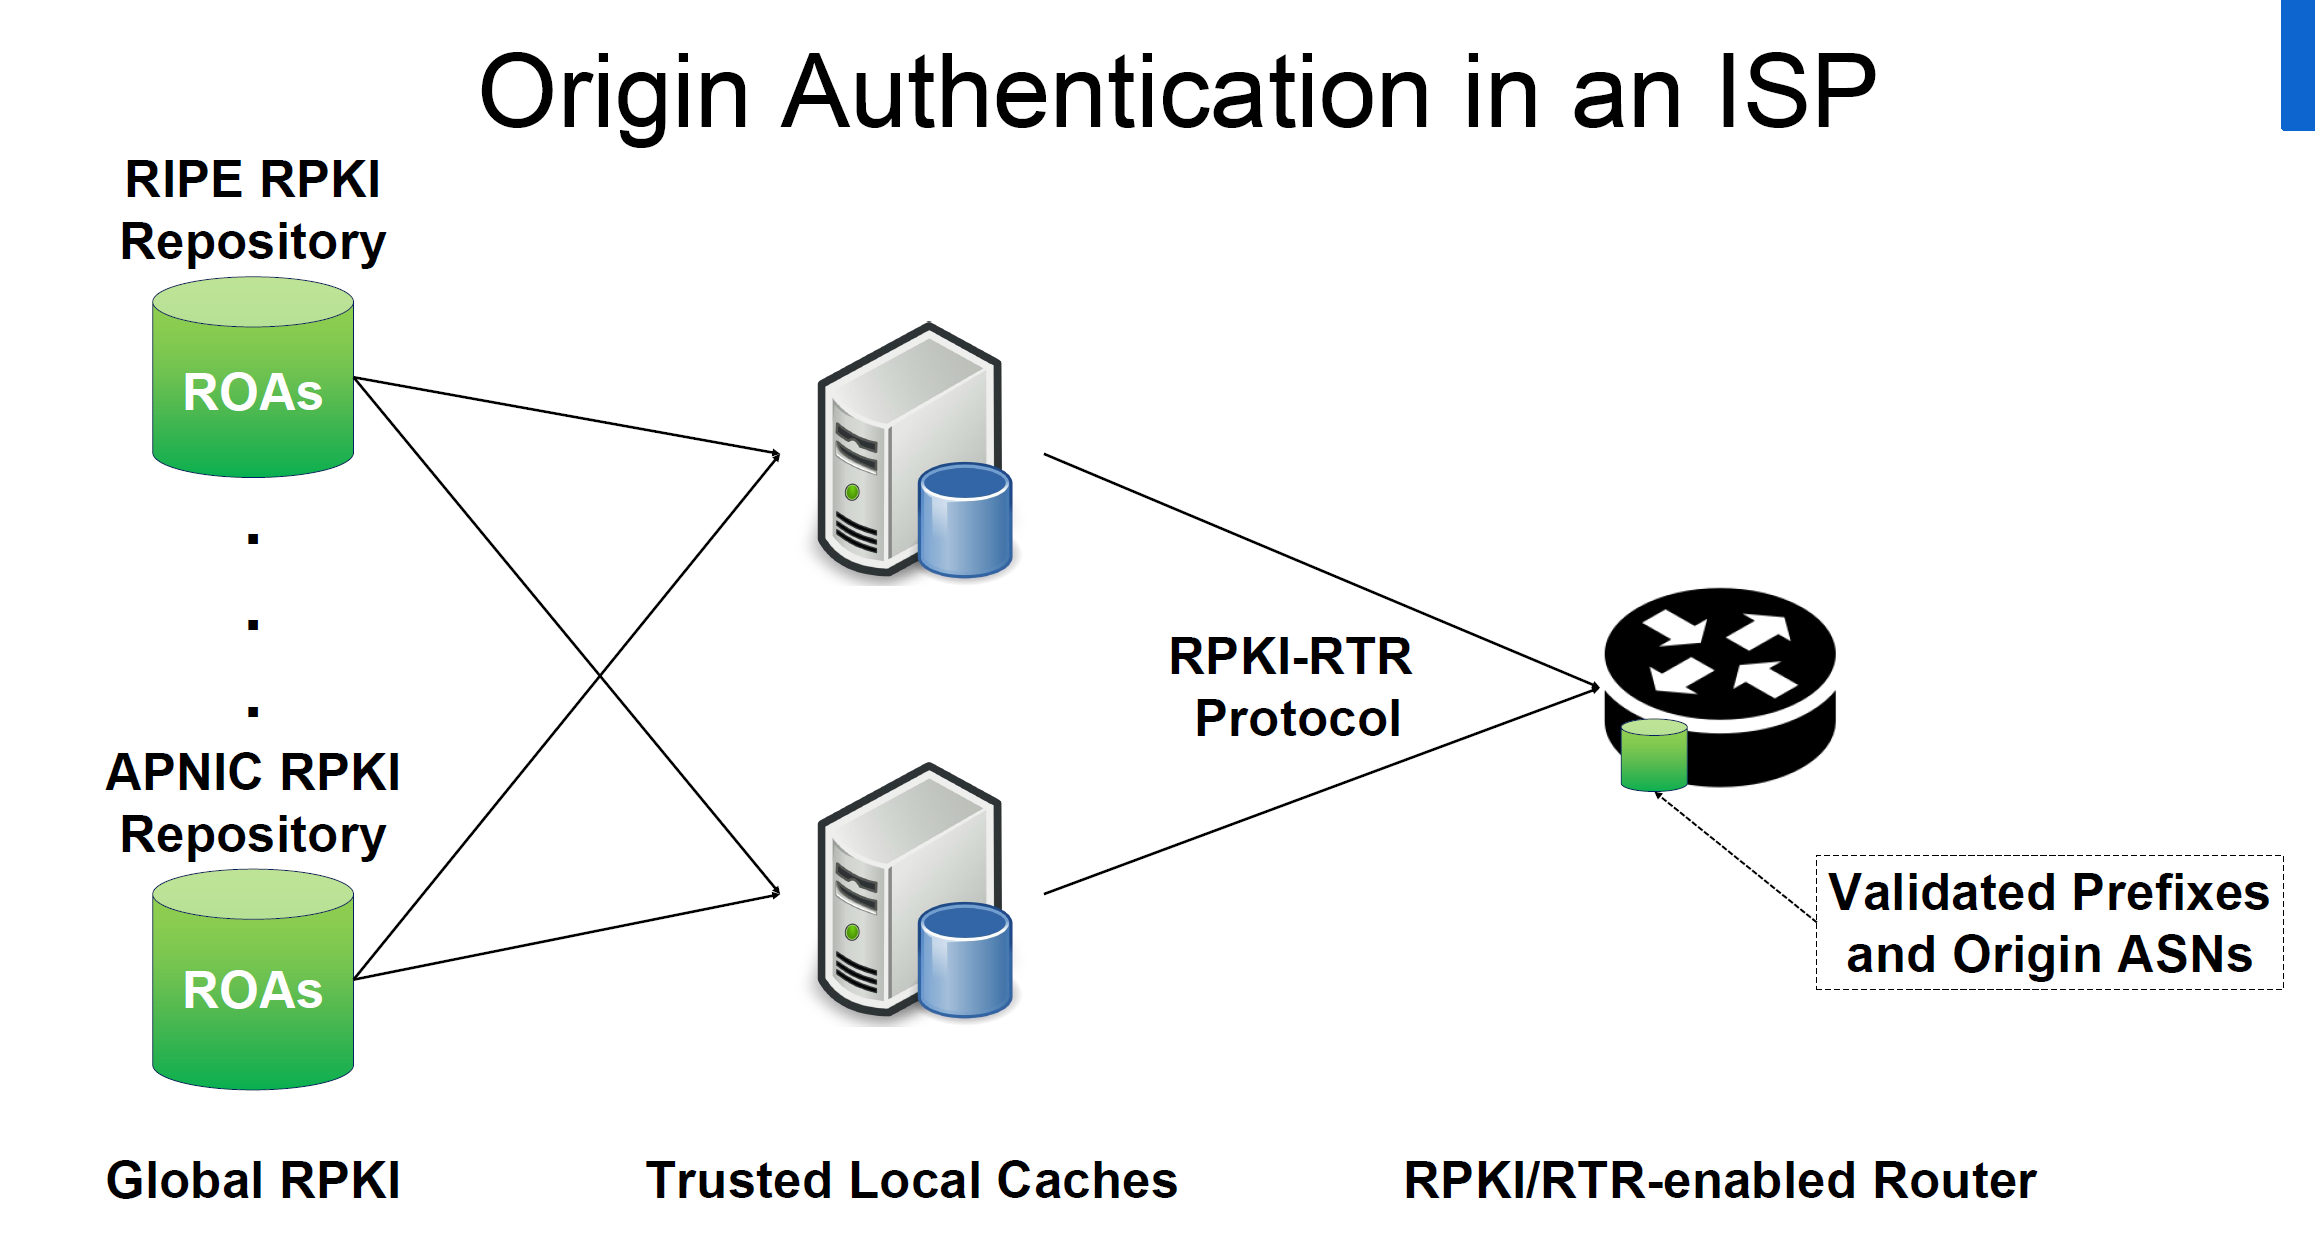
\includegraphics[width=\linewidth]{Figures/BGP_oa.PNG} 
\end{minipage}

\subsubsection{Solution to Problem 2: BGPsec}

In order to prevent the problem of ASes illegitimately appending themselves to AS paths, we need to secure the AS-path attribute, which prevents crafting a valid origin on path and path poisoning. BGPsec is trying to achieve this through Origin authentication and cryptographic signatures.\\
BGPsec signs received update message to prove that path was correctly updated and includes the next AS in the signature. This way, BGPsec can validate that the AS path indicates the order ASes were traversed and that no intermediate ASes were added or removed. RPKI is used to verify AS key material (as in origin authentication).\\

\begin{minipage}{\linewidth}
    \centering      
    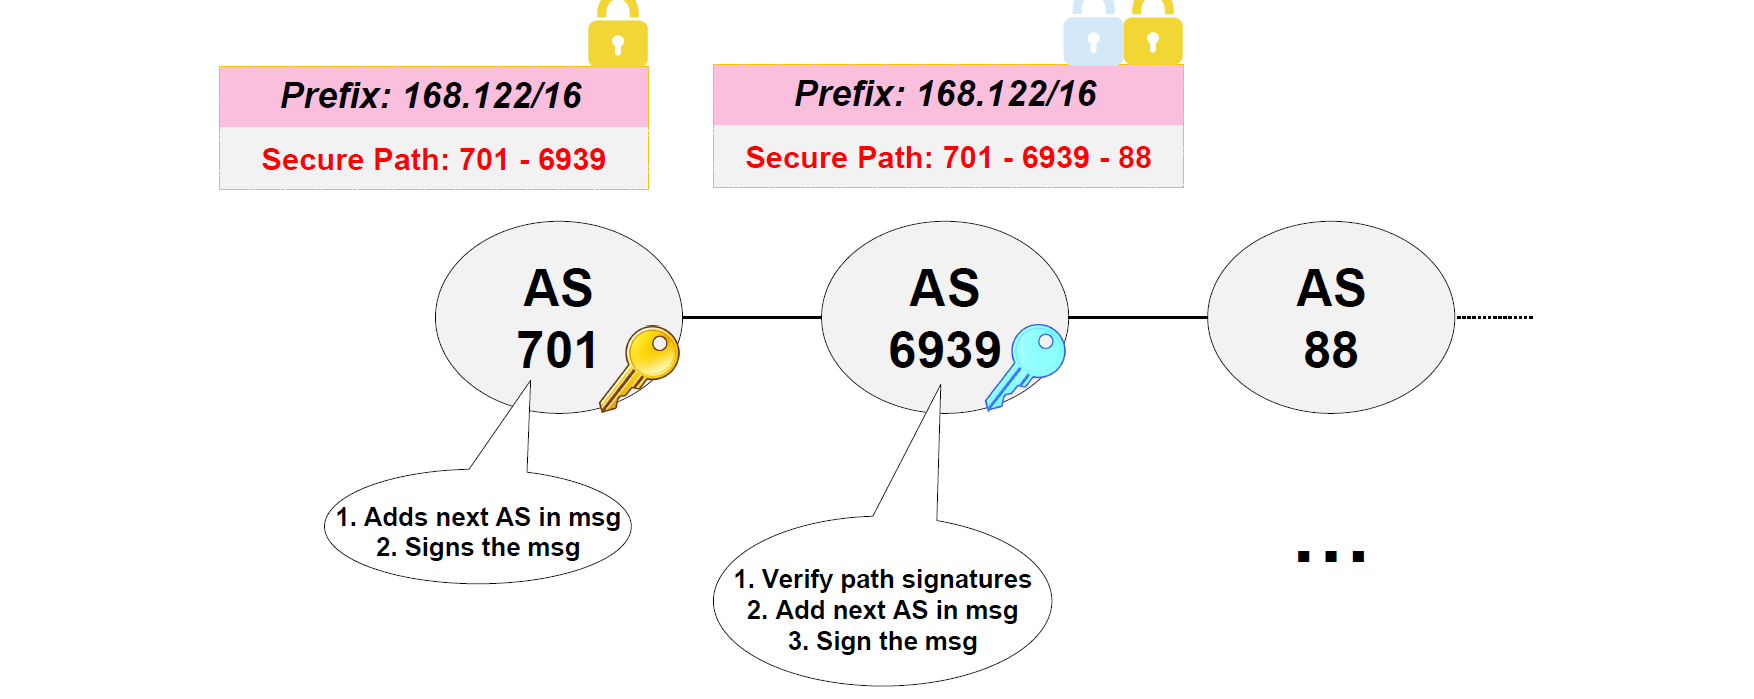
\includegraphics[width=\linewidth]{Figures/BGP_bgpsec.PNG} 
\end{minipage}

Example: AS 701 send out advertisement and signs msg with its privatekey. AS 6939 can verify the signature (pubKey of AS 701) and add the next AS to the path and again sign the message. ASes always need include the next AS on the path and then sign - otherwise there would be no link between ASes and only individual ASes are secured but not the linking between them.

\paragraph{Problems with BGPsec:}
\begin{itemize}
	\item Insecure ASes use legacy BGP, and secure ASes must accept legacy insecure routes $\rightarrow$ \textit{protocol downgrade attacks}: If operators don’t prioritize security, an attacker can just use legacy BGP to announce bogus routes to BGPsec neighbors.
	\item Routing policies can interact in ways that can cause BGP wedgies.
	\item \textit{Performance degradation}: Prefix aggregation no longer possible, since you can't sign a prefix owned by someone else. Real-time signature and validation. Slower convergence.
	\subitem $\rightarrow$ \textit{BGPsec does not scale}
\end{itemize}

\paragraph{Other Approaches: Extensive Monitoring}
\begin{itemize}
    \item Monitoring BGP update messages and use past history.
    \item Out-of-band detection mechanism
\end{itemize}

\subsubsection{Path-End Validation: Deployable Routing Security}

Important observation: AS paths today are very short! Average AS-level path length is only 3-4 hops. The basic idea is to have something between origin authentication and BGPsec. Path-End Validation tries to reduce overhead of BGPsec.\\

\begin{itemize}
	\item Origin Authentication with RPKI secures only the announced prefix. This way, no AS can announce a prefix it does not own.
	\item Path-end Validation secures the first hop	from originator to its provider. This way, no AS can simply append itself after the first AS on the AS path. Why does this work: you can still append yourself after two ASes. \textit{But} this makes the AS path rather long and thus less attractive.
\end{itemize}

This has several advantages over full BGPsec: Lower overhead, requires no cooperation from other ASes, no full deployment necessary, stronger incentive for early adopters.
